% Dedicated source for the cover and 11 main slides, without an appendix.
% Copied from soaring_ctrw_visual_with_appendix.tex on 2026-10-08.
% Compile from this directory: latexmk -pdf soaring_ctrw_visual_11slides.tex
% Figures are shared through the assets/ directory.
% New plots show analytic model results or explicitly illustrative trajectories.
% Original Monte Carlo figures and calibration are reused without rerunning fits.
\documentclass[10pt,aspectratio=169]{beamer}
\usepackage[utf8]{inputenc}
\usepackage[T1]{fontenc}
\usepackage[english]{babel}
\usepackage{mathpazo}
\usefonttheme{serif}
\usepackage{amsmath,amssymb,bm,graphicx,booktabs,array,microtype}
\usepackage{tikz}
\usetikzlibrary{arrows.meta}
\graphicspath{{assets/}}
\definecolor{pisablue}{RGB}{74,96,121}
\definecolor{accent}{RGB}{26,118,179}
\definecolor{tcol}{RGB}{31,80,160}
\definecolor{scol}{RGB}{200,60,50}
\definecolor{ccol}{RGB}{30,140,70}
\definecolor{muted}{RGB}{90,98,105}
\definecolor{pcol}{RGB}{195,120,17}
\setbeamercolor{normal text}{fg=black,bg=white}
\setbeamercolor{structure}{fg=pisablue}
\setbeamercolor{frametitle}{fg=white,bg=pisablue}
\setbeamercolor{alerted text}{fg=accent}
\setbeamertemplate{navigation symbols}{}
\setbeamertemplate{footline}{\vspace{0.12cm}}
\setbeamersize{text margin left=0.70cm,text margin right=0.70cm}
\newcommand{\slidenumber}{\insertframenumber/11}
\setbeamertemplate{frametitle}{%
\nointerlineskip
\begin{beamercolorbox}[wd=\paperwidth,ht=0.74cm,dp=0.23cm,leftskip=0.32cm,rightskip=0.38cm]{frametitle}
\raisebox{-0.14cm}{
\includegraphics[height=0.68cm]{cherubino_white.png}}%
\hspace{0.20cm}{\large\insertframetitle}\hfill{\small\slidenumber}
\end{beamercolorbox}}
\setbeamertemplate{itemize item}{\color{pisablue}\small\textbullet}
\newcommand{\kw}[1]{\textcolor{accent}{\textbf{#1}}}
\newcommand{\vxy}{v_{xy}}
\newcommand{\sth}{\sigma_\theta}
\newcommand{\ehat}{\hat{\mathbf e}}
\newcommand{\Tav}{\langle T_{\mathrm{cyc}}\rangle}
\newcommand{\notefoot}[1]{\par\vfill{\fontsize{7.4}{9}\selectfont\color{muted}#1\par}}
\newcommand{\takeaway}[1]{\par\medskip{\color{accent}\textbf{#1}}\par}
\newcommand{\compactdisplays}{\setlength{\abovedisplayskip}{6pt}\setlength{\belowdisplayskip}{6pt}\setlength{\abovedisplayshortskip}{3pt}\setlength{\belowdisplayshortskip}{3pt}}
\apptocmd{\normalsize}{\compactdisplays}{}{}
\apptocmd{\small}{\compactdisplays}{}{}
\hypersetup{pdftitle={Soaring CTRW: phases, persistence and the asymptotic question},pdfauthor={},pdfsubject={Eleven main slides with title, October 2026}}
\begin{document}
\hypersetup{pdftitle={How directional persistence shapes the Hurst-exponent crossover of thermal soaring flights},pdfauthor={}}


\begin{frame}[plain,noframenumbering]
\vfill
{\color{pisablue}\fontsize{25}{31}\selectfont\bfseries
How directional persistence shapes\\[3pt]
the Hurst-exponent crossover\\[3pt]
of thermal soaring flights\par}
\vspace{0.7cm}
{\large\color{muted}A cycle-based CTRW for cross-country soaring\par}
\vfill
\end{frame}

\begin{frame}[t]{Soaring flight as a sequence of three phases}
\vspace{0.08cm}

\textbf{Target:} the observed $\mathrm{MSD}\propto t^{1.76}$ and its collapse across aircraft classes.
\begin{center}
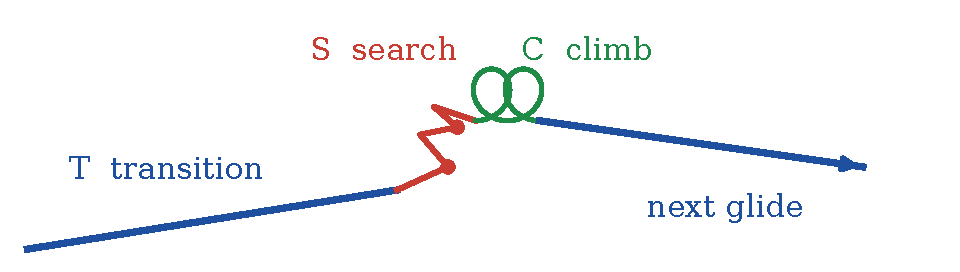
\includegraphics[width=.95\textwidth,height=2.55cm,keepaspectratio]{cycle_trajectory.pdf}
\end{center}
\vspace{-0.18cm}
\begin{columns}[T,onlytextwidth]
\begin{column}{.62\textwidth}
\textbf{We choose Lomax} durations for
\textcolor{tcol}{\textbf{T}} and \textcolor{scol}{\textbf{S}}, as they appear to describe Vilpellet et al.'s empirical survival curves:
\[
P(\tau^X>t)=\left(1+\frac{t}{\tau_0^X}\right)^{-\mu_X},\quad X=T,S.
\]
\end{column}
\begin{column}{.35\textwidth}
We model \textcolor{ccol}{\textbf{C}} with an \textbf{exponential} duration:
\[
P(\tau^C>t)=e^{-t/(110\,\mathrm{s})}.
\]
\end{column}
\end{columns}
\medskip
The chosen parameters have $\mu_T,\mu_S>2$: the cycle clock has finite mean and variance.
\takeaway{The memory between cycles resides in the glide direction.}
\notefoot{Trajectory: schematic. Independent phase durations, i.i.d. across cycles. Empirical inputs: Vilpellet, Darmon and Benzaquen (2026), arXiv:2601.01293.}
\end{frame}

\begin{frame}[t]{Angular diffusion links one glide to the next}
\vspace{0.16cm}
\[
\boxed{\theta_{n+1}=\theta_n+\eta_n\pmod{2\pi},\qquad
\eta_n\overset{\mathrm{i.i.d.}}{\sim}\mathcal N(0,\sth^2)}
\]
\begin{center}
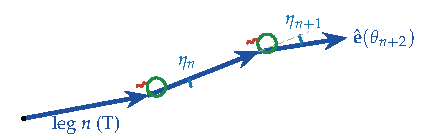
\includegraphics[width=.70\textwidth,height=2.30cm,keepaspectratio]{angular_walk.pdf}
\end{center}
\vspace{-0.15cm}
\[
C(k)=\langle\ehat(\theta_{n+k})\!\cdot\!\ehat(\theta_n)\rangle
=e^{-k\sth^2/2}=\rho^k,\qquad n_c=\frac{2}{\sth^2}.
\]
\medskip
\textbf{$k$ counts successive glides, after segmentation.} It is a cycle lag, not a time lag in seconds.
\medskip

At fixed speed, $\mathbf v_n=\vxy\ehat(\theta_n)$, so
$C(k)=\langle\mathbf v_{n+k}\cdot\mathbf v_n\rangle/\vxy^2$.
\notefoot{$\theta_0$ is uniform. Glide length $\ell_n=\vxy\tau_n^T$ is independent of headings. One glide is ballistic: $\delta_T^2(\Delta)=\vxy^2\Delta^2$. S and C have independent, isotropic local angles.}
\end{frame}

\begin{frame}[t]{Search: long turning waits slow spatial exploration}
\vspace{0.13cm}
\begin{columns}[T,onlytextwidth]
\begin{column}{.52\textwidth}
\centering
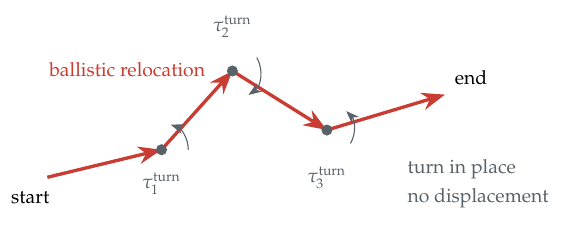
\begin{tikzpicture}[x=1cm,y=1cm,>=Stealth,font=\scriptsize]
\useasboundingbox (-.25,-.35) rectangle (6.4,2.1);
\coordinate (p0) at (0,.20);
\coordinate (p1) at (1.45,.55);
\coordinate (p2) at (2.35,1.55);
\coordinate (p3) at (3.55,.80);
\coordinate (p4) at (5.05,1.25);
\draw[scol,very thick,->] (p0)--(p1);
\draw[scol,very thick,->] (p1)--(p2);
\draw[scol,very thick,->] (p2)--(p3);
\draw[scol,very thick,->] (p3)--(p4);
\foreach \p in {p1,p2,p3}{\fill[muted] (\p) circle (2pt);}
\draw[muted,->] (1.79,.55) arc[start angle=0,end angle=70,radius=.34];
\draw[muted,->] (2.66,1.72) arc[start angle=30,end angle=-55,radius=.36];
\draw[muted,->] (3.85,.63) arc[start angle=-30,end angle=45,radius=.34];
\node[anchor=north,muted] at (1.45,.38) {$\tau^{\rm turn}_1$};
\node[anchor=south,muted] at (2.35,1.85) {$\tau^{\rm turn}_2$};
\node[anchor=north,muted] at (3.55,.45) {$\tau^{\rm turn}_3$};
\node[anchor=south west,scol] at (-.1,1.35) {ballistic relocation};
\node[anchor=north west,muted] at (4.45,.55) {turn in place};
\node[anchor=north west,muted] at (4.45,.18) {no displacement};
\node[anchor=north east] at (.15,.14) {start};
\node[anchor=south west] at (5.05,1.25) {end};
\end{tikzpicture}\par
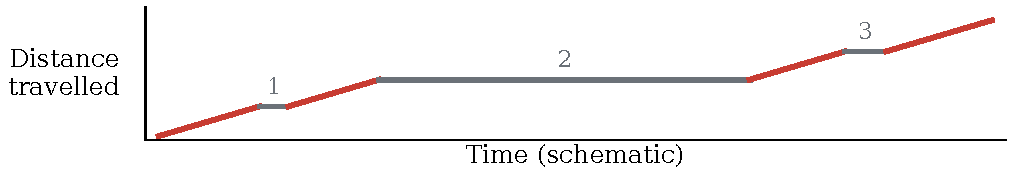
\includegraphics[width=.95\textwidth,height=1.20cm,keepaspectratio]{search_clock_wide.pdf}\par
\raggedright
\medskip
\textbf{MSD within a search episode}
\[
\delta_S^2(\Delta)\simeq
\begin{cases}
u_S^2\Delta^2 & \text{short lag},\\
K_S\Delta^{\alpha_S} & \text{after decorrelation}.
\end{cases}
\]
\end{column}
\begin{column}{.44\textwidth}
\textcolor{scol}{\textbf{Short ballistic relocations}}
\[
\tau^{\mathrm b}\sim\mathrm{Exp}(1/\tau_b),\qquad\tau_b=10\,\mathrm{s}.
\]
\medskip
\textcolor{scol}{\textbf{Mittag--Leffler turning waits}}
\[
P(\tau^{\mathrm{turn}}>t)
=E_{\alpha_S}\!\left[-(t/\tau_{\mathrm{turn}})^{\alpha_S}\right].
\]
No net displacement during a wait.
\medskip

$\alpha_S=0.6,\ 0.6,\ 0.4$\\
for para., hang gliders, sailplanes.
\end{column}
\end{columns}
\takeaway{The renewal clock sets the subdiffusive exponent.}
\notefoot{Schematic path and clock. Curved arrows show turns at fixed position. Turning update: $\psi_{j+1}=\psi_j+\epsilon_j\Omega_S\tau_j^{\mathrm{turn}}$, with $P(\epsilon_j=\pm1)=1/2$. An independent Lomax duration truncates the episode.}
\end{frame}

\begin{frame}[t]{Climb: circling produces a plateau, drift restores growth}
\vspace{0.10cm}
\[
\mathbf x_C(t)=r_0(\cos(\omega t+\phi),\sin(\omega t+\phi))
+\mathbf v_{\mathrm{drift}}t.
\]
\begin{center}
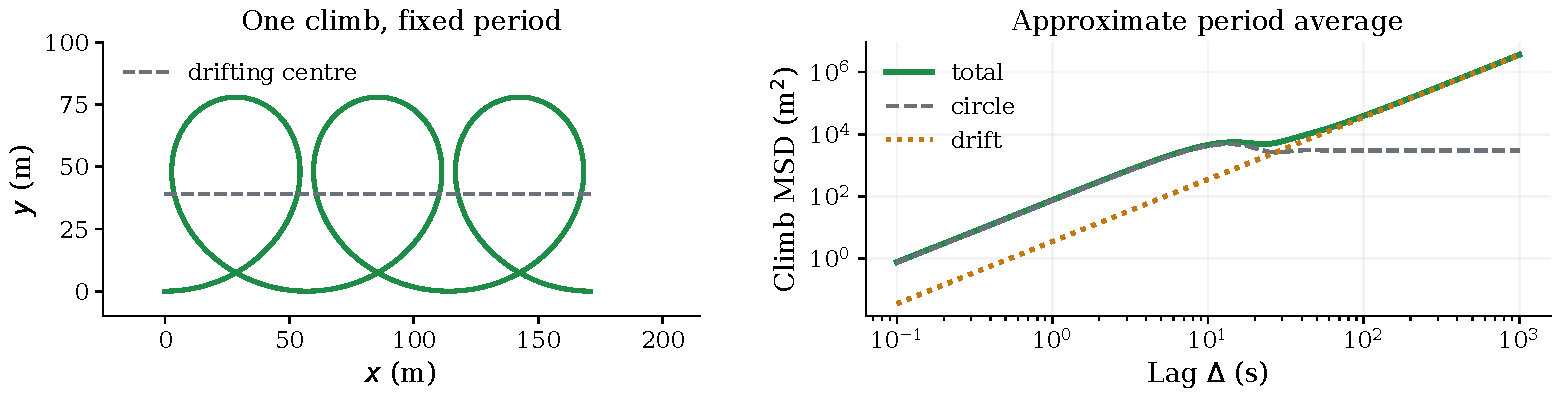
\includegraphics[width=.95\textwidth,height=3.60cm,keepaspectratio]{climb_mechanism.pdf}
\end{center}
\vspace{-0.14cm}
\[
\delta_C^2(\Delta)\simeq
\underbrace{2r_0^2[1-e^{-\sigma_\omega^2\Delta^2/2}\cos(\bar\omega\Delta)]}_{\text{circle + period dispersion}}
\quad+\quad\underbrace{v_{\mathrm{drift}}^2\Delta^2}_{\text{drift}}.
\]
\smallskip
\small
$T_{\mathrm{turn}}\sim\mathcal N(\bar T,\sigma_T^2)$, clipped at $0.2\bar T$.
Orbital phase and drift direction are independent and uniform.
\notefoot{Illustration: paraglider parameters. $\bar\omega=2\pi/\bar T$, $\sigma_\omega\simeq\bar\omega\sigma_T/\bar T$. The closed form is a first-order period-dispersion approximation. The exact period average matches Monte Carlo. Short-lag errors can reach a factor of two for sailplanes.}
\end{frame}

\begin{frame}[t]{Three displacements, one persistent contribution}
\setlength{\abovedisplayskip}{4pt}\setlength{\belowdisplayskip}{4pt}
\vspace{-0.40cm}
\[
\mathbf X_N=
\underbrace{\sum_{n=1}^N\ell_n\ehat(\theta_n)}_{\textcolor{tcol}{\text{transition}}}
+\underbrace{\sum_{n=1}^N\Delta\mathbf x_n^S}_{\textcolor{scol}{\text{search}}}
+\underbrace{\sum_{n=1}^N\Delta\mathbf x_n^C}_{\textcolor{ccol}{\text{climb}}}.
\]
\smallskip
\begin{columns}[T,onlytextwidth]
\begin{column}{.48\textwidth}
\textcolor{tcol}{\textbf{MSD of transition glides}}
\[
M_T(N)=\underbrace{N\operatorname{Var}(\ell)}_{\text{diffusive}}
+\underbrace{\langle\ell\rangle^2G_N}_{\text{coherent}}.
\]
\end{column}
\begin{column}{.48\textwidth}
\textcolor{muted}{\textbf{Search and climb add linearly}}
\[
M_S(N)+M_C(N)=N(\Sigma_S+\Sigma_C).
\]
\end{column}
\end{columns}
\smallskip
\[
G_N\equiv N+2\sum_{k=1}^{N-1}(N-k)C(k),\qquad
C(k)=\rho^k,\quad \rho=e^{-\sth^2/2}.
\]
\smallskip
\[
\boxed{M_N=\mathcal A G_N+\mathcal B N},\qquad
\mathcal A=\langle\ell\rangle^2,\quad
\mathcal B=\operatorname{Var}(\ell)+\Sigma_S+\Sigma_C.
\]
\smallskip
S and C are isotropic and independent across episodes and from T. Their cross terms vanish.
\takeaway{Local search subdiffusion becomes a diffusive contribution across cycles.}
\notefoot{$\Sigma_X=\langle|\Delta\mathbf x_n^X|^2\rangle<\infty$ averages complete episodes over their durations. \underline{For the fitted inputs, $\operatorname{Var}(\ell)$ supplies more than 97\% of $\mathcal B$.}}
\end{frame}

\begin{frame}[t]{A persistent random walk crosses over to diffusion}
\vspace{0.05cm}
\[
G_N=N\frac{1+\rho}{1-\rho}
-\frac{2\rho(1-\rho^N)}{(1-\rho)^2},\qquad \rho=e^{-\sth^2/2}.
\]
\begin{columns}[c,onlytextwidth]
\begin{column}{.62\textwidth}
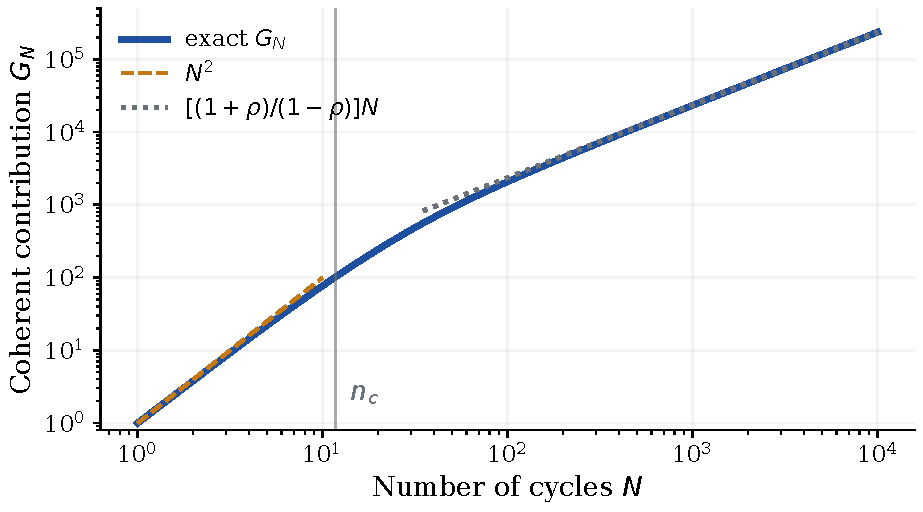
\includegraphics[width=\textwidth,height=4.20cm,keepaspectratio]{persistent_limits.pdf}
\end{column}
\begin{column}{.34\textwidth}
\textbf{Few cycles: $N\ll n_c$}
\[
G_N\simeq N^2.
\]
Aligned legs add coherently.
\medskip

\textbf{Many cycles: $N\gg n_c$}
\[
G_N\simeq\frac{1+\rho}{1-\rho}N.
\]
The long-time limit has $H=1/2$.
\end{column}
\end{columns}
\takeaway{Finite windows can display $H\simeq0.88$ during the crossover.}
\notefoot{Exact in cycle count. $n_c=2/\sth^2$ and $t_c\simeq n_c\Tav$. Illustration: $\sth=0.412$ rad. The total MSD also contains $\mathcal B N$; ballistic scaling requires the coherent term to dominate.}
\end{frame}

\begin{frame}[t]{One fitted angular spread controls the crossover}
\vspace{0.12cm}
\textbf{Calibration target:} $H_{\mathrm{fit}}=0.88$ over lags $10$--$7000$ s.
\medskip
\begin{columns}[c,onlytextwidth]
\begin{column}{.57\textwidth}
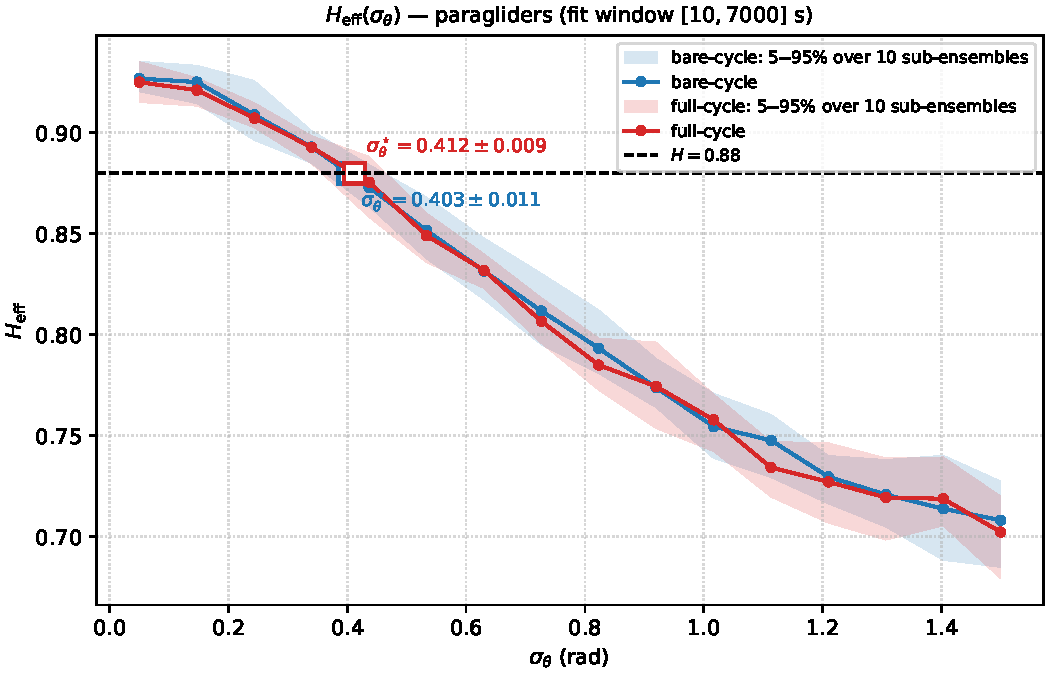
\includegraphics[width=\textwidth,height=4.10cm,keepaspectratio]{estimate_sigma_theta_paragliders_overlay.pdf}

\end{column}
\begin{column}{.39\textwidth}
\small
\renewcommand{\arraystretch}{1.45}
\begin{tabular}{@{}lcc@{}}
\toprule
 & $\sth^\star$ (rad) & $n_c$\\
\midrule
Para. & $0.412\pm.009$ & 11.8\\
Hang gl. & $0.242\pm.005$ & 34.2\\
Sailpl. & $0.556\pm.014$ & 6.5\\
\bottomrule
\end{tabular}
\medskip

$t_c\simeq4.9,\ 15.1,\ 3.1$ ks.
\medskip

Only $\sth$ is fitted per class.\\
Other inputs come from empirical statistics and figures.
\end{column}
\end{columns}
\takeaway{The value $H\simeq0.88$ is a calibration target.}
\notefoot{16 values of $\sth$ in $[0.05,1.5]$ rad. Per value: 2,000 flights of 15,000 s, sampled every second. Log--log OLS on integer lags. Quoted errors: replica standard errors. Figure bands: 5--95\% spread.}
\end{frame}

\begin{frame}[t]{Monte Carlo reproduces the total MSD and its collapse}
\vspace{0.08cm}
\small
Fresh ensemble: 2,000 flights per class, 15,000 s each. MSD measured from each flight's origin.
\smallskip
\begin{columns}[c,onlytextwidth]
\begin{column}{.44\textwidth}
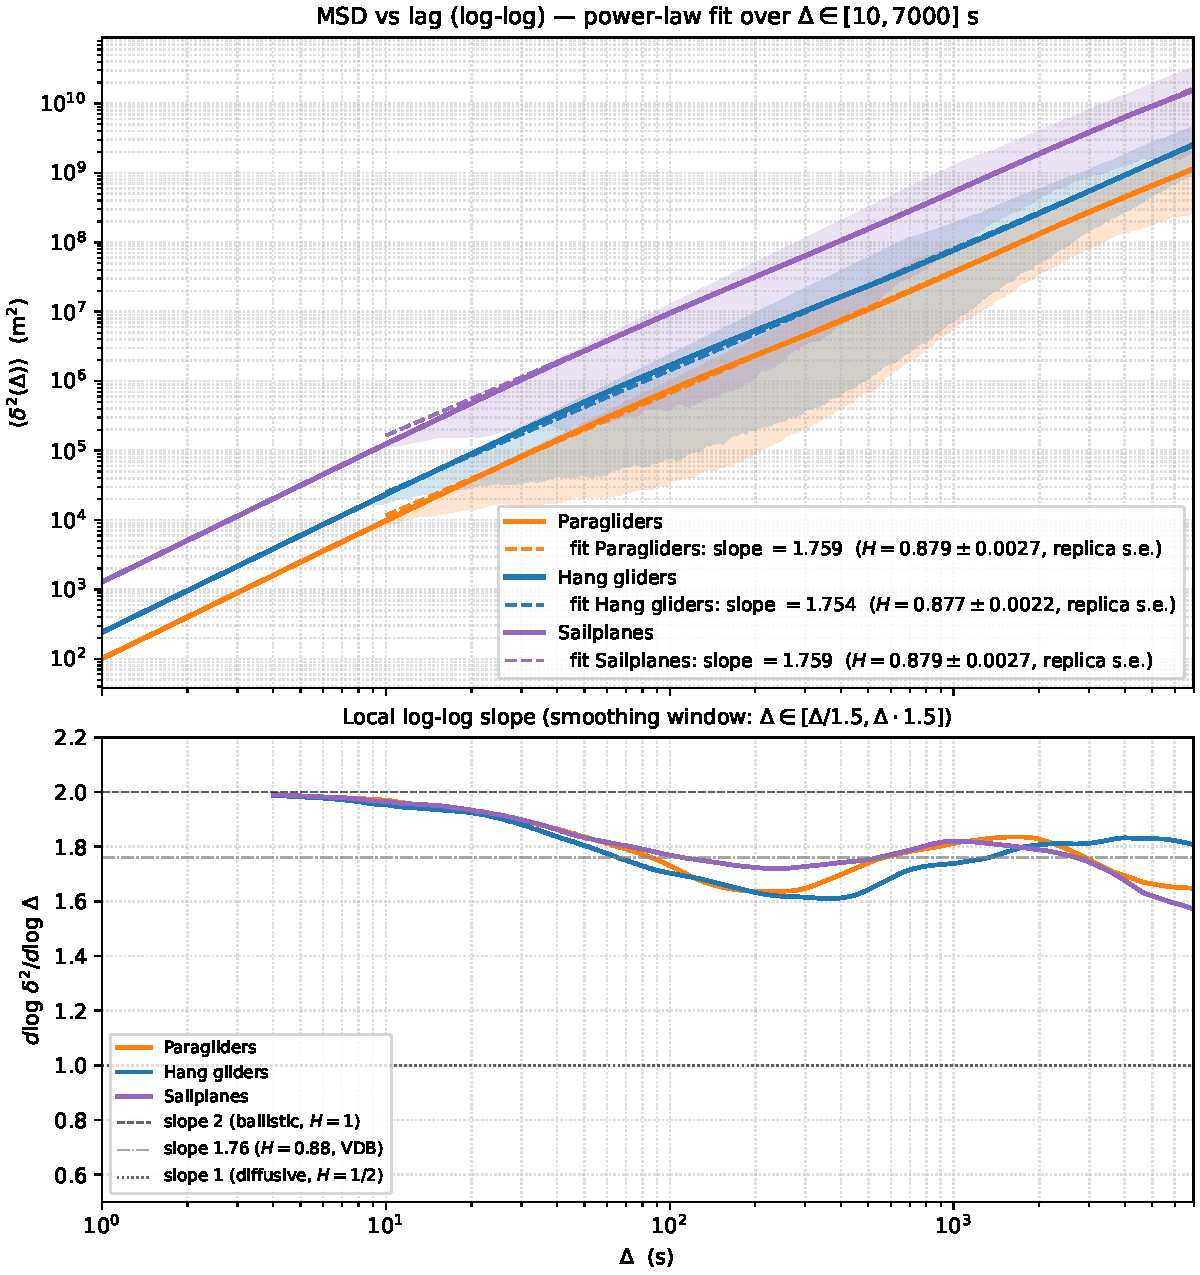
\includegraphics[width=\textwidth,height=5.50cm,keepaspectratio]{msd_all_aircraft_raw.pdf}
\end{column}
\begin{column}{.53\textwidth}
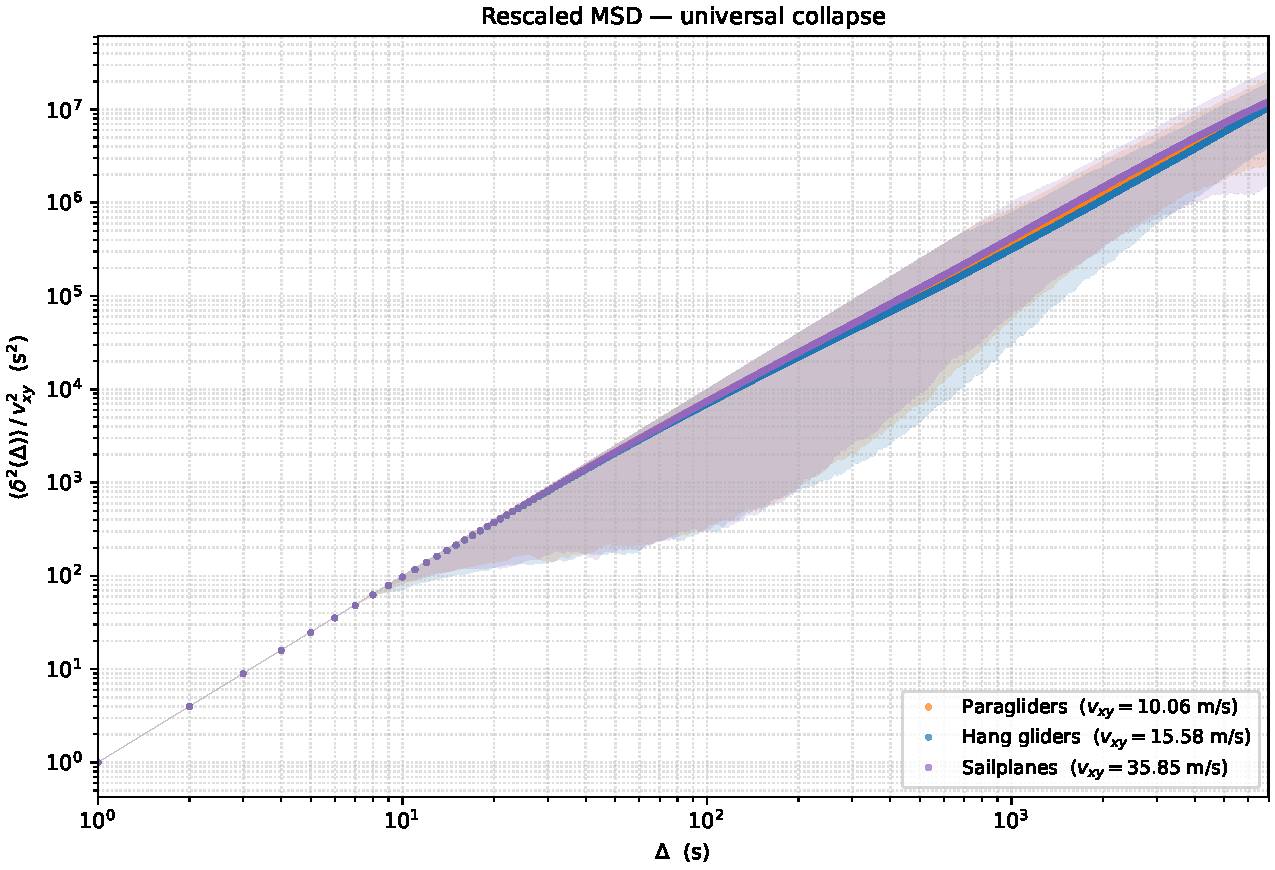
\includegraphics[width=\textwidth,height=4.70cm,keepaspectratio]{msd_all_aircraft_rescaled.pdf}
\par\medskip
\kw{Dividing by $\vxy^2$ collapses the curves.}
\end{column}
\end{columns}
\smallskip
\small
$H_{\mathrm{fit}}=0.879\pm.003,\ 0.877\pm.002,\ 0.879\pm.003$.
\notefoot{Class order: para., hang gliders, sailplanes. Both $\mathcal A$ and the dominant $\operatorname{Var}(\ell)$ scale as $\vxy^2$. Bands show 5--95\% spread of individual squared displacements, not fit uncertainty.}
\end{frame}

\begin{frame}[t]{The phases retain distinct MSD signatures}
\vspace{0.12cm}
\small
Episode-origin MSD, conditioned on the episode lasting at least lag $\Delta$ (seconds).
\begin{center}
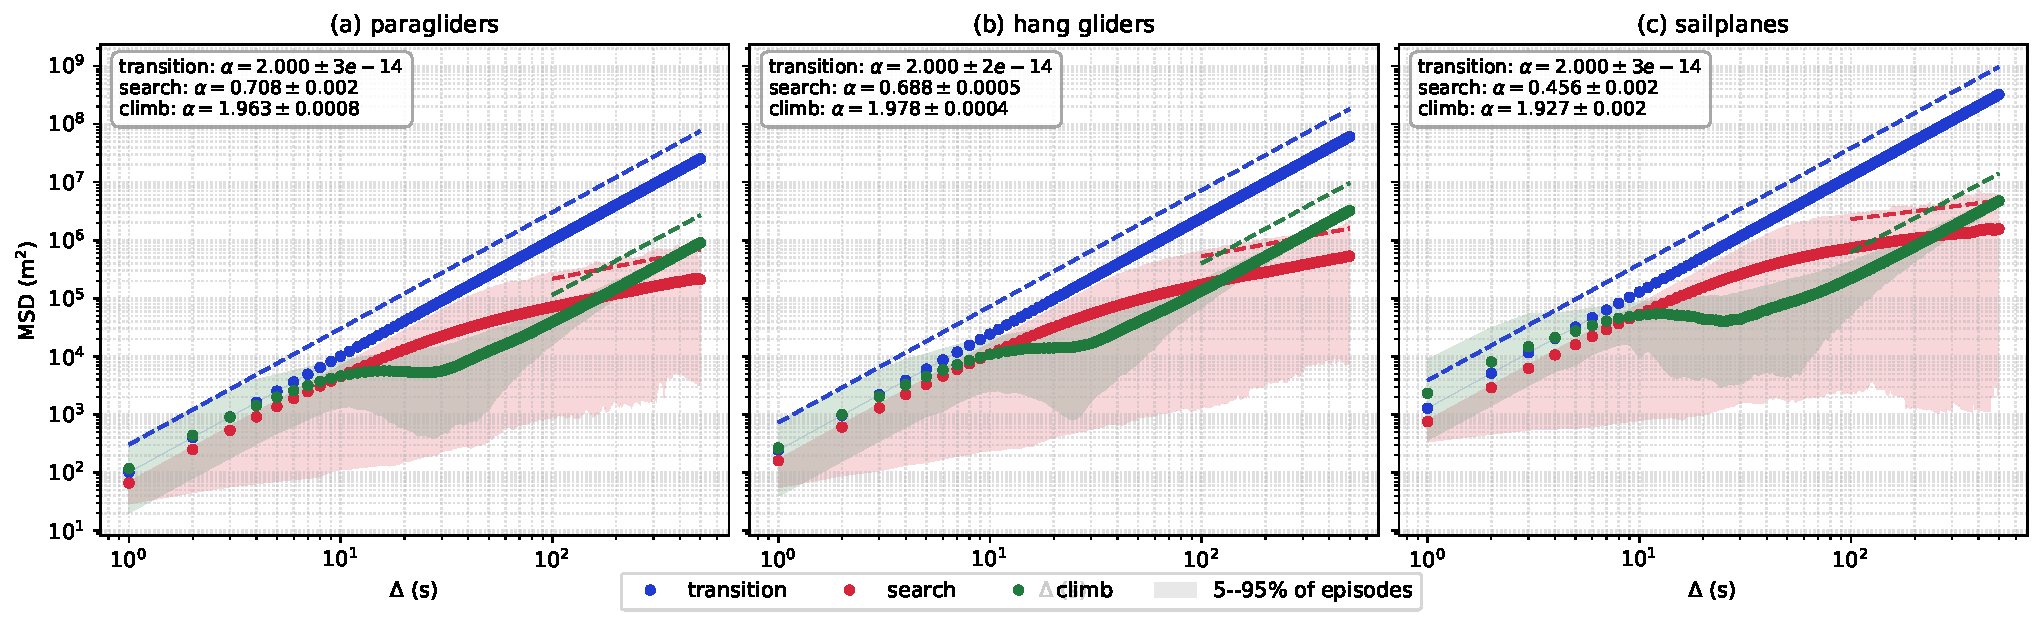
\includegraphics[trim=0 27 0 0,clip,width=.99\textwidth]{per_phase_msd_combined.pdf}
\end{center}
\vspace{-0.1cm}
\begin{columns}[T,onlytextwidth]
\begin{column}{.30\textwidth}
\textcolor{tcol}{\textbf{Transition}}
\medskip

Ballistic: exponent $2$.
\end{column}
\begin{column}{.34\textwidth}
\textcolor{scol}{\textbf{Search}}
\medskip

Subdiffusive: $0.708$,\\$0.688$, $0.456$.
\end{column}
\begin{column}{.30\textwidth}
\textcolor{ccol}{\textbf{Climb}}
\medskip

Dip, then drift:\\$1.96$, $1.98$, $1.93$.
\end{column}
\end{columns}
\par\medskip\kw{No individual phase gives exponent $1.76$.}
\notefoot{Monte Carlo: 2,000 flights of 50 cycles per class. Search inputs $\alpha_S=0.6,0.6,0.4$; finite episodes limit the asymptotic regime. Exponents follow panel order and plotted fit annotations. Bands: 5--95\% episode spread.}
\end{frame}

\begin{frame}[t]{A simpler model keeps glide, waiting and angular memory}
\vspace{0.16cm}
Merge search and climb into a single waiting time:
\[
\boxed{W_n=\tau_n^S+\tau_n^C},\qquad
T_{\mathrm{cyc},n}=\tau_n^T+W_n.
\]
\begin{center}
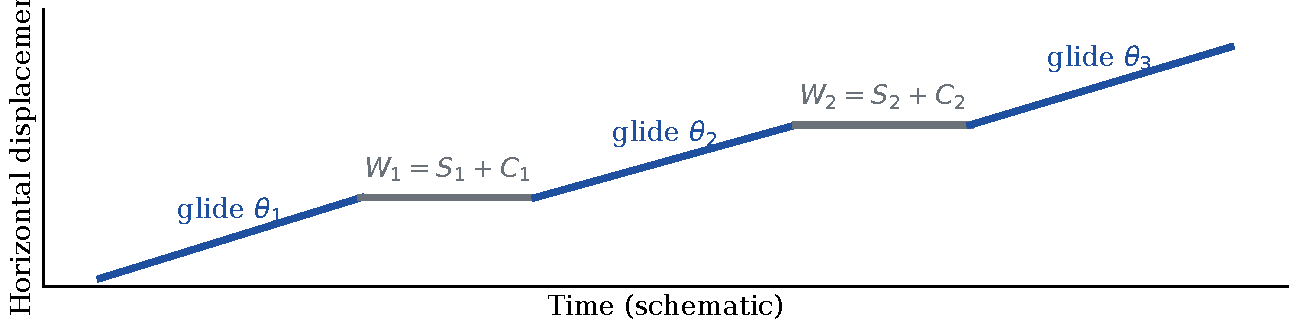
\includegraphics[width=.92\textwidth,height=2.80cm,keepaspectratio]{glide_wait.pdf}
\end{center}
\vspace{-0.10cm}
\begin{columns}[T,onlytextwidth]
\begin{column}{.48\textwidth}
\textbf{Preserve the clock and memory}
\smallskip

Glides are ballistic. Position is fixed during $W_n$. The next glide retains angular memory.
\end{column}
\begin{column}{.48\textwidth}
\textbf{Remove local displacements}
\smallskip

The full MSD differs by $N(\Sigma_S+\Sigma_C)$ at cycle boundaries.
\end{column}
\end{columns}
\takeaway{A large-scale approximation with the same angular transport mechanism.}
\notefoot{$W$ follows the convolution of the search Lomax law and the climb exponential law. Its mean and variance remain finite. This simplification removes S/C phase MSDs and their short-time structure. Plot: schematic horizontal coordinate.}
\end{frame}

\begin{frame}[t]{A non-summable correlation sustains superdiffusion}
\vspace{0.04cm}
\[
M_N=(\mathcal A+\mathcal B)N
+2\mathcal A\sum_{k=1}^{N-1}(N-k)C(k).
\]
\begin{center}
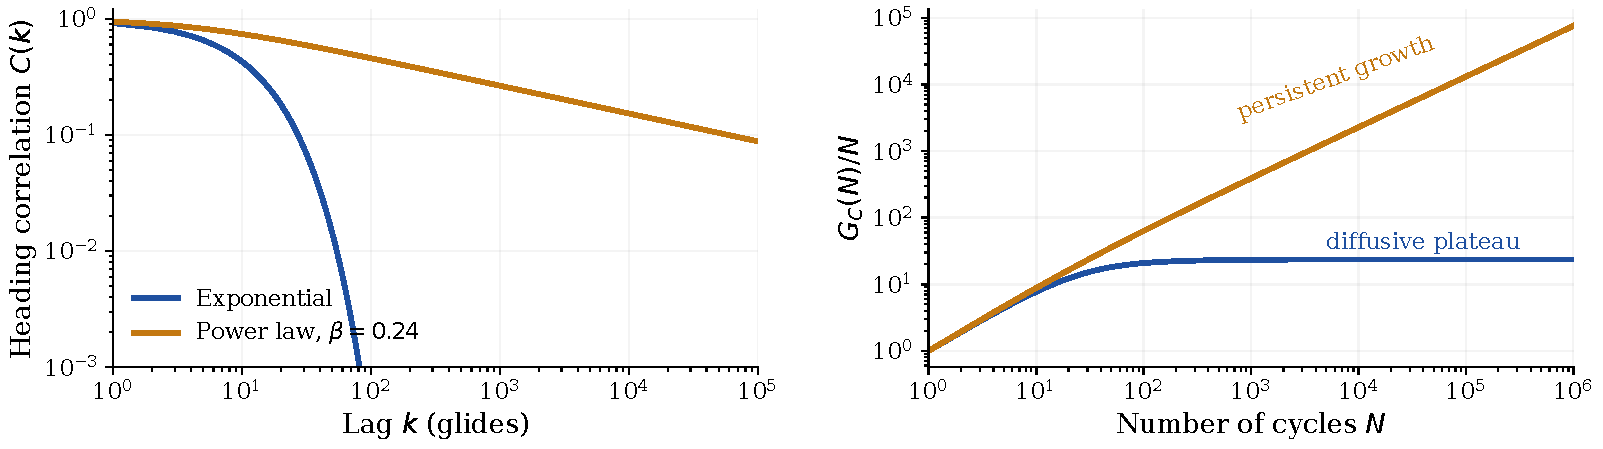
\includegraphics[width=\textwidth,height=3.80cm,keepaspectratio]{correlation_asymptotes.pdf}
\end{center}
\vspace{-0.13cm}
\begin{columns}[T,onlytextwidth]
\begin{column}{.46\textwidth}
\textcolor{pcol}{\textbf{$C(k)\sim c\,k^{-\beta}$, $c>0$, $0<\beta<1$}}
\[
M_N\propto N^{2-\beta},\quad H=1-\frac{\beta}{2}.
\]
\end{column}
\begin{column}{.50\textwidth}
\textbf{Boundary and diffusive cases}\smallskip

$\beta=1$: $M_N\sim N\log N$.\\
$\beta>1$ or exponential: $M_N\propto N$.
\end{column}
\end{columns}

\end{frame}

\end{document}
